\documentclass[14pt]{extarticle}
\usepackage{amsmath}
\usepackage{multicol}
\usepackage{tikz}
\usepackage{tabularx} % in the preamble

\begin{document}


\begin{center}
\begin{tabular}{ c c c }
 
\begin{tikzpicture}
\shade (0,0) circle (.5cm); 
\end{tikzpicture}
 & 
 
 
\begin{tikzpicture}
\shade (0,0) circle (.5cm); 
\end{tikzpicture}

 & cell3 \\ 
 cell4 & cell5 & cell6 \\  
 cell7 & cell8 & cell9    
\end{tabular}
\end{center}


\begin{tikzpicture}
\shade (0,0) rectangle (2,1)
(3,0.5) circle (.5cm); 
\end{tikzpicture}


\begin{tikzpicture}
\shade (0,0) circle (.5cm); 
\end{tikzpicture}

% ....
\begin{tabularx}{\textwidth}{|X|c|}
\hline
\textbf{Code} & \textbf{Diagram} \\
\hline
\texttt{
shade (0,0) circle (2cm); 
} 
&
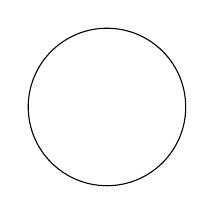
\begin{tikzpicture}
\draw (0,0) circle (1cm); 
\end{tikzpicture}\\
\hline
\end{tabularx}


\end{document}